% !TEX root = ../thesis_main.tex



%%%% --- * --- %%%%	
%\clearpage
%\chapter{Introduction}
\chapter{Background}
\label{intro_chapter}
\label{nuclear_chapter}

\section{An Abbreviated Look at the History of Beta Decay}
\note[tag]{History section needs *all* the citations.}
We consider the historical development of our scientific understanding of beta decay and the nuclear weak force.  This is a historically rich topic, and a full discussion is beyond the scope of this document, however we shall attempt to touch on some highlights.

Radioactivity was first observed in 1896 by Henri Becquerel in uranium, and this landmark discovery set off a flurry of activity in the field~\cite{becquerel1896}.
% With our modern understanding of radioactive decay, we know that this of course could not have been beta decay, but rather a combination of alpha decay and spontaneous fission -- however it was this observation that set the field into motion.  
Ernest Rutherford noted in 1899 that the particles emitted by a sample of uranium could be classified into two groups based on how readily they were absorbed in materials -- alpha particles are easily absorbed, while beta particles are more penetrating~\cite{rutherford1899}.  A third and even more penetrating type of radioactive emission was observed in 1900 by Paul Villard, who made no attempt to give it a name -- but within a few years, Rutherford's naming convention had been applied and this third type of particle became known as a gamma ray~\cite{villard1900}\cite{rutherford1903}.  

When, in 1900, Becquerel measured the charge-to-mass ratio of emitted beta ($\beta^-$) radiation and found that it was the same as that of the electron, he proposed that these must be the same particle~\cite{becquerel1900} (I think.  Also, I think that's the right citation..), and in 1901 (or possibly 1903?) Rutherford and Soddy demonstrated that the processes of alpha and beta decay both transmute the original chemical element into another.  

\note{That arxiv rando claims that the half-life thing was developed or hinted at by 1900 Rutherford, but who the fuck knows?}

\note{Halliday doesn't remember Meitner+Hahn, and says Pauli's thing is 1927, but doesn't give a reference for it.
\\...\\
Also from Halliday:  Yukawa and Sakata first proposed the possibility of (orbital) electron capture in 1935-1936.  (What about Wick in 1934?)
\\...\\
Also-also:  Fermi in 1934 drew an analogy between emission of electrons and neutrinos from nuclei and emission of photons from excited atomic states.... (probably this gets us one step closer to isospin?)
}
\note{I could totes add a reference to Halliday's 1955 textbook (v2).}
\note{Other references to add include that one letter to the collaboration giving values of *things* from Ian Towner, 2011.}
\note{How do I reference a grant proposal?}
\note{separate ref. for the PRL's supp. mat.}
...
\note{I should probably cite Dan's thesis.  And Alexandre's too.}
...
\note{More references to add, for some of the numbers in that text file:
\\...\\
The Branching Ratio from Severijns 2008 ~\cite{SeverijnsTandecki2008} \\
The Probability of electron capture from Severijns 2008 \\
The halflife from Shidling PRC 2014 ~\cite{pshidling} \\
statistical rate function from Severijns 2008 \\
Axial to Vector Ratio from Severijns 2008 \\
Nucleus Dependent Radiative Correction from Severijns 2008 \\
Nuclear Structure Dependent Corrections and isospin symmetry breaking correction from Severijns 2008 \\
Isospin symmetry breaking correction (delta\_C1 + delta\_C2) from Severijns 2008 \\
FT from 0plus to 0plus decay Hardy PRC 2015 (eq. 5) ~\cite{hardytowner2015} (Hardy+Towner) \\
Weak Magnetism from Naviliat-Cuncic 2009 \\
Sign of Rho determined by shell model from Severijns 2008 \\
Average Mass need to calculate parameters as a function of energy Naviliat-Cuncic 2009 (is it~\cite{naviliat2009april}, or~\cite{naviliat2009june}??  No way to know.) \\
Parent Magnetic Moment from von Platen Z. Phys. 244 (1971) ~\cite{vonplaten1971} \\
daughter magnetic moment from from M. Pitt Ph.D. (1992) ~\cite{mpitt1992} \\
Parent quadrupole moment Minamisono PLB 662 (2008) ~\cite{minamisono2008quadrupole} \\
daughter quadrupole moment Klein NPA 607 (1996) ~\cite{klein1996} \\
??? for electron mass (wikipedia) \\
mass of parent 37K taken out of Dan's code mass of 37K \\
daughter mass from ??? \\
Average kinetic energy from Severijns 2008 (is this thing even used??) \\  
"ALPHA", whatever that is:  CODATA 2018 (It's what I think it is.)~\cite{} \\
things from Ian Towner 2013:  all the (reduced) matrix elements and all the coupling constants with quenching corrections.~\cite{itownerCalcs} \\
... \\
Really, this shit can probably can be an appendix.
}

Despite these early successes, in 1911 Lise Meitner and Otto Hahn noticed that beta particles are emitted with a variety of different kinetic energies, and in 1914 James Chadwick demonstrated that energies of emitted beta particles formed a continuous distribution.  The physics community was baffled by the fact that it seemed impossible to predict the energy of a beta particle emitted by a particular process;  if the emitted beta simply took on the difference in energy between the initial and final elements, then surely that should be a fixed amount of energy for a given transition.  Finally in 1930, Wolfgang Pauli proposed that the presence of an additional small, neutral, difficult to detect particle could account for the continuous beta energy spectrum.  He named this particle the ``neutron'' -- though today we refer to that same particle as a ``neutrino,'' and use the name ``neutron'' for an entirely different particle.

\note{alpha and beta decay:
\\
Rutherford, Ernest (1899). “Uranium radiation and the electrical conduction produced by it,” Philosophical Magazine 47, 109-163.
\\...\\
half-life:
\\
Rutherford, Ernest (1900). “A radio-active substance emitted from thorium compounds,” Philosophical Magazine 49, 1-14.
Or, possibly:
\\
Rutherford, Ernest (1906). Radioactive Transformations. London: Constable \& Co.
\\...\\
Transmutations?:
1902, 1903 --- rutherford and soddy.
}
%%%He named this particle a "neutron", though he was referring to the particle we refer to today as the "neutrino".  
%%%
%%%(which he referred to as a "neutron" at the time, though we now call it a neutrino, and use the term "neutron" to describe something else)
%%%
%%%
%%%a neutrino (which he referred to as a "neutron" at the time) 

When Enrico Fermi offered a quantitative description of 



\section{Draft of Intro Section}
\subsection{bullet points.}
Beta Decay:
\begin{itemize}
\item 1931 - Pauli "discovers" neutrinos and is very confused.
\item 1934 - Fermi's Golden Rule to describe the rate of beta decay in terms of transition matrix elements.
\item ...
\item 1956 - Lee and Yang wonder if parity is even conserved in beta decay?  
\item 1957 - C.S. Wu shows that parity isn't conserved.  At all.
\item ???? - turns out it's V-A.
\end{itemize}
Standard Model:
\begin{itemize}
\item ???? - Schwinger 
\item 1959 - Glashow
\item 1964 - Salam and Ward
\item 1967 - Weinberg
\item 1971 - 't Hooft
\item ...
\item 1954 - Yang + Mills  .... huh?
\end{itemize}

Radioactivity:
\begin{itemize}
\item 1896 - Henry Bequerel in Uranium.  Presumably that's alpha decay.
\item 1898 - Thorium is radioactive -- Marie Curie + Gerhard Carl Schmidt, independently.
\item 	 - Curie:  Thorium, polonium, radium -- all radioactive!
\item 1899 - Rutherford notices that there's two types of emissions:  alpha and beta (beta minus).
\item 1900 - Paul Villard discovers gamma rays, doesn't realize they're different?  Or something?
\item 1903 - Rutherford realizes that gamma rays are a fundamentally new thing.
\item ...
\item 1900 - Becquerel realizes beta particles have the same charge-to-mass ratio as electrons, postulates that they're the same thing.
\item 1901 - Rutherford + Soddy show that alpha and beta decay turn elements into different elements.  
\item ...
\item 1911 - Lise Meitner + Otto Hahn:  emitted beta particles come out at many different energies.  Unlike alpha and gamma decays.
\item 1914 - James Chadwick shows that it's a continuous distribution.
...
\item 1930 - Pauli proposes neutrinos (but he called them "neutrons") as a solution to the missing energy problem.
\item 1931 - Fermi calls them neutrinos.  
\item 1933 - Fermi's landmark theory?  Surely it's 1934.
...
\item 1934 - Irène and Frédéric Joliot-Curie discover (induced) beta+ decay.  it got 'em a nobel prize.
\item 1934 - Wick proposes electron capture as a thing.  Yukawa and others maybe have thoughts about that too.
\item 1937 - Luis Alvarez observes electron capture.
\end{itemize}

\subsection{paragraphs}
OK.  This stuff is basically yoinked from Ben's thesis.  And Dan's.  I'll need to re-organize and rephrase the content -- but I want to make sure I get the important points down.  

In 1931, Pauli figured out about neutrinos, because beta decay produced a whole spectrum of beta energies, so there had to be a third body available to carry off some of the energy.  (Dan doesn't cite anyone here)

There's the matrix element, $\mathcal{M}_{fi}$, which connects the initial and final nuclear states, before and after an interaction (decay).  

\bea
\mathcal{M}_{fi} &=& \int \psi_f^* \mathcal{O} \psi_i \textrm{d}V  \;\;\;\; \textrm{(What is $V$??  Pretty sure it's phase space volume.)}, 
\eea 
which goes with Fermi's Golden Rule (or at least one of them):
\bea
\Gamma &= \;\; \frac{1}{\tau} \;\; =& \frac{2\pi}{\hbar} \left| \mathcal{M}_{fi} \right|^2 \, \rho(E_f)  \;\;\;\; \textrm{(Why is this formatted weird??)},
\eea
where, as Ben puts it, $\rho(E_f)$ is "the thermodynamic density of states available at a final energy".  Then he writes down the differential decay rate and cites ~\cite{fermi1934german} 
%\cite{fermi1934english} 
for it, which is in German:
\bea
\frac{\textrm{d}^5 W}{ \textrm{d} \Ebeta \textrm{d}\Omega_\beta \textrm{d}\Omega_\nu } 
&=& \frac{G_F^2}{(2\pi)^5} \pbeta \Ebeta (E_0 - \Ebeta)^2 F_{\pm}(\Ebeta, Z^\prime) \left| \mathcal{M}_{fi} \right|^2
\eea
Anyway, that thing was published in 1934 !  And he assumed the interaction only worked at $0$ distance.  Also, he postulated that the weak force was a vector interaction, and some of it is!  

Later, we collectivelly learned that a better model is to suppose that the interaction is mediated by a massive, charged $W^+$ or $W^-$ particle.  Also, it's pretty heavy, and Ben totally gives the mass so he can cite the dudes who compile that stuff, but there's a new version now.  As of 2018, we have $m_W = 80.379(12)$\,GeV/$c^2$ ~\cite{pdg2018}.  The point is, the fact that it's so massive means that the approximation of $0$ distance was pretty good, since the larger mass implies that the interaction can only occur at short range.

So we're going to require that $\mathcal{O}$ must behave under a Lorentz transformation.  You can construct operators with the correct form out of Dirac $\gamma$-matrices, and you get scalar, pseudoscalar, vector, axial vector, and tensor couplings.  potentially.  Anything else would just reduce to linear combinations of those, so those ones span the space.  Some of those respect parity, and some don't.  

Up until 1956, it was common wisdowm that weak interactions should respect parity, but there was really no evidence for it.  Lee and Yang formulate a more general description of beta decay, with all the Lorentz symmetry respecting operators, and only some of those obey parity~\cite{LeeYang}.  It was an open question, then, whether parity should be respected in the nuclear weak interaction -- but not for long, because C.S. Wu tested it out in 1957~\cite{wu}.  The result of the experiment is that not only is parity *not* conserved, it's (sometimes) *maximally* not conserved!  Neat!  Nobody would have expected it.

Ben points out that they thought it was scalars and tensors at first, and cites some people(\cite{RustadRuby1955tensor}\cite{BurgyEpstein1957scalartensor}), but frankly, I can't access those articles and I thought there was more evidence for it than that.  Also, the one article is published before Madame Wu's, so idk what to make of that.

Ben points out that the $V-A$ form of the interaction means that parity is *maximally* violated, however he also says that $A$ has $+$ and $V$ has $-$ parity.

Anyway.  We're maximally parity violating, and when we describe this in modern terminology, we would say that the $W^{\pm}$ particles only couple to negative helicity (left-handed) leptons, or positive helicity antimatter leptons (anti-leptons).

Also, chirality as a concept.  It's an intuitively straightforward concept when your particle is going at the speed of light.  So, for a massless neutrino, if it has a negative chirality, that means that its spin vector is pointed opposite to its direction of motion.  

Also-also, the fundamental property is chirality, not helicity.  Helicity can be flipped by a simple Lorentz boost.  But because we're talking about an interaction, there is some sense in which this defines a rest frame for us.   ....is this even the correct way to think about it?  I think it has to be fine.

So anyway, we have lots of evidence for the $V-A$ form of interactions.  (Ben doesn't cite anyone for this).  But other forms of the interaction could be in there too.  And at this point, Ben just assumes the Standard Model and goes with it.

-- -- -- -- -- -- 

Within the present understanding of physics, there are four fundamental forces governing the interactions of particles with one another:  electromagnetism, the nuclear weak force, the nuclear strong force, and gravity.  These four forces are considered different by virtue of the fact that each one couples to a different type of charge, is mediated by a different type of particle, and therefore has potentially different behaviour at varying length scales.  The most familiar example of this is a comparison between the forces of electromagnetism and gravity.  While the electromagnetic force couples to both positive and negative electric charges, and can therefore create both attractive and repulsive forces, the gravitational force couples only to (positive) mass, and the result is a force that is only attractive and never repulsive.  Both forces are mediated by massless particles (the photon and graviton, respectively), which implies that the strength of the two forces must fall off at the same rate as the distance between interacting bodies is increased.

Attempting to unify the four forces within a single theoretical framework has been a major focus of later 20th- and early 21st century physics to date, however the effort has thus far been met with some limited success.


\note{OK, how/when did they do electroweak unification, and who did it?  What about the full SM, incorporating the strong force too?}
\note{Schwinger does renormalization, which makes QED go. Glashow~\cite{Glashow1959} extends it to the Z boson.  But now it's not renormalizable.  Salam and Ward~\cite{SalamWard1964} did a similar thing, but independently.   Then Weinberg (1967) did it but didn't know what to do with Z bosons~\cite{Weinberg1967}.  Until later.  Or something.  Then, 't Hooft (1971) proved that this thing was normalizable even with massive gauge bosons~\cite{thooft1971}.  Or at least, that's how Wikipedia describes it.  Also, in the end, electroweak unification was based on Yang-Mills (1954)~\cite{YangMills1954}, but their theory didn't really get that much attention initially because it was just a lot of boring math, and they couldn't figure out how to something something symmetry breaking.}

%Attempts to unify the four forces within a single model have been a major focus of 20th- and 21st century physics, }

%%%Both are mediated by massless particles (the photon and graviton, respectively)
%%%Because these are both mediated by massless particles (the photon and graviton, respectively), their behaviour 

The nuclear weak force is one of four fundamental forces described within physics.  It mediates the process of beta decay, which is of particular interest to us here.  Although beta decay is generally well understood, it presents a unique opportunity for precision measurements to search for physics beyond the Standard Model within the Weak coupling.\aside[jbn]{Standard Model -> standard model of particle physics (often denoted here "SM"). 
\\
The standard model is ...
\\...\\
Weak -> weak.
\\...\\
This of course is the place where Georg wants more for orientation.
}
By observing the kinematics and angular correlations involved in the decay process, one gains access to a wealth of information about the form of the operators mediating the decay.  

\note[done]{JB says:  Chapters 1.1 and 1.2 look fine.
\\
My only comment is to ask where the Fermi "singlet" and "triplet" came from, referring to coupling of the lepton spins.
I have not seen this-- it could be fine, yes, I don't know.
}
\note[jb1]{JB:  The Gamow-Teller operator sigma dot tau refers to nucleon spins, not lepton spins, i.e. the nucleon spin can flip, but that doesn't tell me about this lepton rule either way.
You correctly state the lepton and antilepton chirality farther down.
}

\note[jbn]{John's suggestions for fixing the stuff that Georg wanted fixed -- that giant email.
i) Among the necessary technical corrections, there's a solid request for more background info. I think you know what to do.
\\...\\
A large thing is some kind of extra qualitative description of what the SM is. You could do that qualitatively without any trouble.
}
\note[jbn, nolist]{
You might point out some part of this:
\begin{itemize}
	\item the charged weak interaction you're writing down predates the Weinberg-Salam model by more than a decade. The version you've written down assumes protons and neutrons are fundamental particles.
	\item The exchange boson is much heavier in mass than the energy and momentum in the decay, so it can be approximated by an interaction with zero range. 
	\begin{itemize}
		\item Fermi did that very early on, 
		\item and Gamow and Teller added a process that change the nucleon spin. 
		\item Lee and Yang, which you cite, added the possible currents with different Lorentz transformations (do you mention that since any further combination of Dirac matrices can be reduced to these, so they span the space), and the possibility of parity violation by writing out helicity projections for the leptons. I.e. Lee and Yang assumed some fields (the nucleons and leptons) and a general interaction preserving the symmetries of the theory, which by definition is then an effective field theory.
	\end{itemize}
	\item Feynman and Gell-Mann's 1958 paper is the one that postulated V-A, again a decade before Weinberg-Salam, and they did this by making analogies between the boson exchanged and the photon, i.e. an analogy between the charged weak interaction and the electromagnetic current, so you could cite them instead of saying "SM predicts everything"
\end{itemize}
People had assumed there was a massive boson exchanged for a very long time.
\\
What Weinberg (and, independently, Salam) did was come up with a consistent mathematical theory of massive bosons, incorporating Yang Mills gauge theory (looks like E\&M but with nonabelian operators) to do that, and the result was the weak neutral interaction prediction.
}

\section{Beta Decay within the Standard Model}
A nucleus undergoing beta decay converts one of its protons (neutrons) into a neutron (proton), and simultaneously emits a lepton and anti-lepton.  The daughter nucleon remains bound in place of its parent, and the overall electric charge of the nucleus is changed by -1 (+1), with the extra charge being carried away by the anti-lepton (lepton).  In particular, at the nucleon level, three beta decay processes are possible:
\bea
	p &\rightarrow& n + e^+ + \nu_e        \label{eq:betaplus_decay} \\
	n &\rightarrow& p + e^- + \bar{\nu}_e, \label{eq:betaminus_decay}  \\
	p + e^- &\rightarrow& n + \nu_e        \label{eq:electroncapture}
\eea
where the processes described in Eqs.~\ref{eq:betaplus_decay} and~\ref{eq:electroncapture} are energetically disallowed for an unbound proton, however there is no similar requirement for Eq.~\ref{eq:betaminus_decay}.
~\aside[jbn]{Eqs. ~\ref{eq:betaplus_decay} and ~\ref{eq:electroncapture} are energetically disallowed for an unbound proton, but allowed energetically when bound in nuclei as in 37K decay.}
\note[jbn]{Electron capture decay of Eq. 1.3 is calculated to be an 0.080\% branch compared to positron decay in 37K decay (Table VII of N. Severijns, M. Tandecki, T. Phalet, and I.S. Towner)~\cite{SeverijnsTandecki2008}, an important correction when interpreting the total decay rate of 37K to determine the theoretical prediction for 37K Abeta  (P.D. Shidling, R.S. Behling, B. Fenker, J.C. Hardy, V.E. Iacob, M. Mehlman, H.I. Park, B.T. Roeder, D. Melconian Phys Rev C 98 015502 (2018)~\cite{shidling2018}; A. Ozmetin, D.G. Melconian, V.E. Iacob, P. Shidling, V.S. Kolhinen, D.J. McClain, M. Nasser, B. Schroeder, B. Roeder, H. Park, M. Anholm, A.J. Saastamoinen, APS DNP Abstract KF.00005 2020 ``Improving the ft value of 37K via a precision measurement of the branching ratio'')~\cite{ozmetin2020}.
}
Limiting the focus of this discussion to Eq.~\ref{eq:betaplus_decay}, we note that this expression provides no information at all about the momenta or spin of the outgoing daughter particles.  This behaviour is governed by the form of the Weak coupling that mediates the decay.  

Within the field of nuclear physics, it is common to classify beta decay processes as being either ``Allowed'' or ``Forbidden''~\aside[jbn]{don't capatalize "Allowed" and "Forbidden."
The quotes are justified.} (sometimes with an associated number to describe the extent to which it is Forbidden), where Forbidden processes are generally suppressed but not truly forbidden.  In an Allowed transition, the positron and anti-neutrino are treated as being created at the nuclear centre, and as a result they may not carry away any \emph{orbital} angular momentum.  However, since the outgoing leptons both have spin $S=1/2$, it is still possible for the total nuclear angular momentum, $J$, to be changed in an Allowed decay.  This implies that an Allowed transition must \emph{always} change the total nuclear angular momentum by either $0$ or $\pm1$.  
~\note[jbn]{First forbidden decay emits leptons with total orbital angular momentum 1, changing the nuclear parity-- suppressed in a long-wavelength approximation ~ ((beta momentum)/(hbar c))$^2$ or about two orders of magnitude. This is one reason decays to negative-parity excited states of 37K are so small (Fig.~\ref{fig:nuclearleveldiagram}).
}

The Allowed decays traditionally are further separated into a ``Fermi'' singlet~\aside[jbn]{singlet in lepton spin} in which there is no change to nuclear angular momentum ($\Delta J = 0$) and therefore the two leptons are required to have anti-parallel spins, and a ``Gamow-Teller'' triplet~\cite{severijns_beck_cuncic_2006}, where the projection of the nuclear angular momentum is changed by $\pm1$.%, and so the two lepton spins must be aligned in parallel to one another under the Allowed approximation.

This implies that the total nuclear angular momentum is changed by $\Delta J = \{0, \pm1\}$ during a Gamow-Teller transition.  A mixed transition is also possible, however we note that the $J_i = J_f = 0$ decays must always be pure Fermi transitions, because there is no way to produce this result from two outgoing leptons with parallel spins.~\cite{krane}~\cite{wong1990}~\cite{severijns_beck_cuncic_2006}.

Given the differing behaviour within the angular momenta of the daughters in Fermi and Gamow-Teller transitions, it is perhaps not suprising that that the \emph{linear} momenta of the outgoing particles should also follow a different set of distributions in these two cases.  At the level of the Weak~\aside[jbn]{Don't capitalize Weak anywhere, either. You can keep quotes around the first "weak", I guess.} coupling, Fermi- and Gamow-Teller~\aside[jbn]{you should indeed capitalize Fermi and Gamow-Teller because these are people.} transitions are governed by different operators, with the Fermi interaction mediated by a so-called ``vector'' ($V$) coupling, and the Gamow-Teller interaction mediated by an ``axial-vector'' ($A$) coupling.
~\note[jbn]{The vector and axial-vector couplings refer to Lorentz transformation of the Lagrangian terms involved, which we come to next.}

% and therefore carry angular momentum, the total nuclear angular momentum may still be changed.
%Allowed transitions, in which the decay may not  as either ``Fermi'' decays, 
%Since the topic of this work involves the Beta+ decay process of Eq.~\ref{eq:betaplus_decay}, that will be the primary focus in the discussion of beta decay that follows.
%we will focus primarily on that in the discussion that follows.
%We will focus primarily on the process of Eq.~\ref{eq:betaplus_decay}


%%\note{The TRIUMF Neutral Atom Trap (TRINAT) offers an experimental set-up which is uniquely suited to precision tests of Standard Model beta decay physics.  Radioactive ions are delivered from the ISAC beamline and neutralized before being trapped in the first of two magneto-optical traps (MOTs).  Approximately once per second, atoms from the first MOT are transferred to the second, where their decay products can be observed with significantly less background than would have been possible in the first trap (see Figure~\ref{fig:doublemot}).  The transfer methodology is discussed in some detail in a paper by Swanson et al~\cite{swanson}. (The point is that this eliminates background from the decays of other stuff.  Or the same stuff.  Stuff that's not centered at the trap.)}

%\note[jb1]{JB on the contents of Chapter 1:  \\
%Move what you have in 1.1 and 1.3 to the first section of Chapter 2, and otherwise omit Chapter 1.}


% ~\cite{wu}
% ~\cite{LeeYang}
%\aside{Did I even get this right?  Is the phase angle really what makes it left-handed? \\ JB says:  \\ ... \\ Relative sign.  look at the quark-lepton Lagrangian, which has $(1 \pm \gamma_5)$ } 
%Any such behaviour, should it be present, would necessarily be a non-dominant contribution to the interaction, however it cannot be entirely ruled out.  
%Any such behaviour with would necessarily be only 
% cannot be entirely ruled out, and the search for physical interactions beyond the Standard Model (BSM) is an active field of research. \aside{cite someone?}  
%, and our observable is mostly sensitive to scalar (S) and tensor (T) couplings.  
%\note{According to present limits, these couplings would have to be pretty small relative to the ($V$) and ($A$) couplings.}


%%%%%\note[jb1]{from JB on the contents of Chapter 1:
%%%%%%\\
%%%%%%With three changes:
%%%%%%\\ ... \\
%%%%%%1)"and we shall be interested especially in scalar (S) and tensor (T) couplings." -> "our observable is mostly sensitive to scalar (S) and tensor (T) couplings."
%%%%%\\ ...\\
%%%%%2)
%%%%%"These couplings all refer to parameters in a Lagrangian that takes the
%%%%%relativistic inner product of a current for the lepton with a current for the
%%%%%proton or neutron.
%%%%%The resulting Lagrangian must be a scalar under Lorentz transformations, so
%%%%%these currents must have transformations like these V,A,S, and T and be
%%%%%combined into a scalar."
%%%%%\\...\\
%%%%%3) Add one reference to the latest review:
%%%%%\\
%%%%%Adam Falkowski, Martín González-Alonso, Oscar Naviliat-Cuncic. Comprehensive analysis of beta
%%%%%decays within and beyond the Standard Model. Journal of High Energy Physics, Springer, 2021, 04,
%%%%%pp.126. 10.1007/JHEP04(2021)126.
%%%%%\\
%%%%%Here it is!~\cite{Falkowski2021}.
%%%%%\\ ... \\
%%%%%You have time for nothing else.
%%%%%}

%%%%%\note[jb1]{Me:  \\ Is a `phase angle' really what makes it left-handed? \\.\\ JB says:  \\ Relative sign.  look at the quark-lepton Lagrangian, which has $(1 \pm \gamma_5)$ }

%%%%%\bluetodo{Need to figure out how the exotic couplings actually work, mathematically.  What the fuck does ``$(V-A)$'' even *mean*?  IIRC John wants a brief mention of $\gamma_5$'s and $\gamma_\mu$'s, and probably a brief mention of whatever mumble-mumble group is mumble-mumble represented or something.
%%%%%\\
%%%%%...
%%%%%\\
%%%%%JB says:
%%%%%\\
%%%%%the current transforms like a Lorentz scalar or tensor -- this does not refer to the angular momentum.
%%%%%\\
%%%%%If you write down the Lagrangian for beta decay, that's eough. All these things refer to the structure of the Lagrangian. The theory considers all possible Lorentz transformations of the currents. 
%%%%%\\
%%%%%Please don't talk about SU(2)xU(1) for electroweak unification. It's textbook material that's beyond the scope.
%%%%%}

%%%%%%\note{ The general form of the weak interaction Hamiltonian is: \\
%%%%%%\bea
%%%%%%\hat{H}_{\mathrm{weak}} &=& \sum_{i=S,P,V,A,T} \left( {\bar{\psi}}_p {\mathcal O}^i \psi_n \right) \left( C_i \bar{\psi}_e {\mathcal O}_i \psi_\nu + C_i^\prime \bar{\psi}_e {\mathcal O}_i \gamma^5 \psi_\nu \right) + H.C.
%%%%%%\eea
%%%%%%with
%%%%%%\bea
%%%%%%{\mathcal O}_S &=& 1            \\
%%%%%%{\mathcal O}_P &=& \gamma^5     \\
%%%%%%{\mathcal O}_V &=& \gamma_\mu    \\
%%%%%%{\mathcal O}_A &=& i \gamma_\mu \gamma^5  \\
%%%%%%{\mathcal O}_T &=& \frac{-i}{2\sqrt{2}} \left( \gamma_\mu \gamma_\nu - \gamma_\nu \gamma_\mu \right)
%%%%%%\eea
%%%%%%\\
%%%%%%It's from here:  ~\cite{hong_sternberg_garcia}.
%%%%%%\\ 
%%%%%%Also, unclear what subscripts $p,n,e,\nu$ mean.  I could guess/assume, but....
%%%%%%}



%%%% --- * --- %%%%	
%
%
%
%
%
%
%
%%%% --- * --- %%%%	
%\section{Motivation}
\section{A Generalized Description of the Weak Interaction}
%\section{Background}
%\section{Motivation}
%\greycomment{The nuclear Weak force is one of four fundamental forces described within physics.  It mediates the process of beta decay, which is of particular interest to us here.  Although beta decay is generally well understood, it presents a unique opportunity for precision measurements to search for physics beyond the Standard Model within the Weak coupling.  By observing the kinematics and angular correlations involved in the decay process, one gains access to a wealth of information about the form of the operators mediating the decay.}

According to the predictions of the Standard Model~\aside[jbn]{standard model} (SM), the Weak force involves only vector ($V$) and axial-vector ($A$) couplings, where a relative sign within the quark-lepton Lagrangian produces the left-handed ``$(V-A)$'' form of the interaction in maximal violation of parity.  In terms of physical behaviour, one consequence of this model is that ``regular matter'' leptons emerge from a Weak interaction with left-handed chirality, while antimatter leptons emerge with right-handed chirality. Any deviation from this behavior would be indicative of ``new'' or ``exotic'' (i.e., not previously discovered) physics.
~\aside[jbn]{"new" -> new
\\
"exotic" -> exotic. 
\\...\\
You define them right away. There is no need for air quotes. You should seriously think about never using air quotes, but use them as an indication to you that you need to write down more clarifying words instead.}

There exists an extensive body of experimental evidence to demonstrate that the above model is overall a very good description of the beta decay process~\cite{wu}.  Despite the success of the $(V-A)$ model, there are still certain lingering questions that must be addressed by precision measurements.  Any deviation from maximal parity violation (i.e., a ``$(V+A)$'' contribution to the Weak force) would be of great interest to the community, as would the presence of certain other exotic couplings, such as the so-called Scalar ($S$) and Tensor ($T$) interactions.  Any such behaviour beyond the Standard Model (BSM) would represent a non-dominant contribution to the interaction, however the possibility cannot be entirely ruled out.  
~\note[jbn]{This is where I'm suggesting a little more explanation of Lee and Yang, and  V-A from Feynman and Gell-Mann}

%Lee-Yang 
The generalized nucleon-level Lagrangian to describe the Weak interaction including BSM behaviour is given by:
% !TEX root = ../thesis_main.tex
%
%
%%%% --- * --- %%%%	
\bea
{\mathcal L} &=& - \bar{p}\gamma^\mu n \left( C_V^+ \bar{e} \gamma_\mu \nu_L + C_V^- \bar{e} \gamma_\mu \nu_R \right) -\bar{p}\gamma^\mu \gamma_5 n \left( C_A^+ \bar{e} \gamma_\mu \nu_L - C_A^- \bar{e} \gamma_\mu \nu_R \right) 
\nonumber\\
&& - \bar{p} n \left( C_S^+ \bar{e} \nu_L + C_S^- \bar{e} \nu_R \right) - \frac{1}{2} \bar{p} \sigma^{\mu\nu} n \left( C_T^+ \bar{e} \sigma_{\mu \nu} \nu_L + C_T^- \bar{e} \sigma_{\mu\nu} \nu_R \right) 
\nonumber\\
&& + \bar{p}\gamma_5 n \left( C_P^+ \bar{e} \nu_L - C_P^- \bar{e} \nu_{R} \right) + \textrm{H.C.}, 
\label{eq:lee_yang_lagrangian} 
\eea
%%%%  \label{eq:lee_yang_lagrangian} 
where the coupling constants $C_X^{\pm}$ (with $X=\{V,A,S,T,P\}$) are written in such a way as to separate out the left-handed ($C_X^{+}$) and right-handed ($C_X^{-}$) components from one another, and the neutrino fields $\nu_{L,R}$ are given a similar treatment.  
%the left- and right-handed components of both the coupling constants and neutrino fields are separated out from one another, with left-handed couplings $C_X^{+} = $
%coupling constants $C_X^{\pm}$ are written
%$C_X^{+}$ and $C_X^{-}$ describe the left-handed and right-handed (respectively) 
A simple variable transform relates Eq.~\ref{eq:lee_yang_lagrangian} to expressions that are potentially more familiar from the older literature, much of which was written before it had been determined that the Weak force is primarily or entirely left-handed: 
\bea
\nu_{L} &=& \frac{1}{2}\nu \left( 1 + \gamma_5 \right) \\
\nu_{R} &=& \frac{1}{2}\nu \left( 1 - \gamma_5 \right) \\
C_X &=& \frac{1}{2} \left( C_X^+ + C_X^- \right) \\
C_X^\prime &=& \frac{1}{2} \left( C_X^+ - C_X^- \right)
\eea
\note[jbn]{Can you please provide a reference for Eq.~\ref{eq:lee_yang_lagrangian}? I'm now confused about how you can get pure 1+gamma\_5 projections without assuming Cv=Cv' and Ca = +/- Ca' (I forget the convention) so I really think you need to reference this expression rather than derive it.
} 
It can be seen from the form of the Lagrangian that the $V,A,S,T,P$ couplings within are described as such because they \emph{behave} as vectors, axial-vectors, scalars, tensors, and pseudoscalars (respectively) under a Lorentz transform, where the Lagrangian itself must be a scaler both before and after a Lorentz transform~\cite{LeeYang}~\cite{Falkowski2021}~\cite{hong_sternberg_garcia}.
\note[jbn]{(Any quark-lepton pseudoscalar couplings have usually been ignored in beta decay, because they are suppressed by (beta momentum)/(nucleon mass).  Note that more recently it's been pointed out that C\_P is naturally quite large in the nucleon (M. Gonzalez-Alonso and J. Martin Camalich Phys Rev Lett 112 042501 (2014)) and allows for significant constraints from allowed beta decay.)}

%\note[bluetodo]{Seriously, this section needs some citations.  Notably, C.S. Wu~\cite{wu} (done) and Lee+Yang~\cite{LeeYang} (done).  Perhaps also Hong+Sternberg+Garcia~\cite{hong_sternberg_garcia}.  Probably a bunch more people too though.}
%%\note{Write a paragraph about what we're looking for with this experiment.}
%%%\note[done]{John wanted this change (now implemented), but I think the phrasing is unclear now: \\
%%%"and we shall be interested especially in scalar ($S$) and tensor ($T$) couplings." -> "our observable is mostly sensitive to scalar ($S$) and tensor ($T$) couplings."
%%%\\ ... \\
%%%In fact, that sentence is gone now, but I no longer talk about which things we're sensitive to in this section of the intro.}



%%%% --- * --- %%%%	
%
%
%
%
%
%
%
%%%% --- * --- %%%%	
%%%%%%%\section{The Basics of Beta Decay}
%%%%%%%	%\\*
%%%%%%%	%The Fermi description of beta decay can be found in any nuclear physics textbook, but you have to dig slightly harder to understand Gamow-Teller or mixed decays, all of which are relevant here.  
%%%%%%%%Beta decay within the Standard Model is well understood.  \greycomment{At the nucleon level, two processes are possible:
%%%%%%%%\bea
%%%%%%%%	p &\rightarrow& n + e^+ + \bar{\nu}_e  \label{eq:betaplus_decay} \\
%%%%%%%%	n &\rightarrow& p + e^- + \nu_e, \label{eq:betaminus_decay}
%%%%%%%%\eea
%%%%%%%%where Eq.~\ref{eq:betaplus_decay} is energetically disallowed for an unbound proton, however there is no similar requirement for Eq.~\ref{eq:betaminus_decay}.  
%%%%%%%%}
%%%%%%%
%%%%%%%\greycomment{We will limit the scope of this discussion to Allowed transitions, in which a beta decay may not change the \emph{orbital} angular momentum.  However, as the outgoing leptons have spin$=1/2$ and therefore carry angular momentum, the total nuclear angular momentum may still be changed.  Since a beta decay creates \emph{two} new leptons, this implies that the total nuclear angular momentum must always change by either $0$ or $1$ in an Allowed decay ~\cite{krane}.}
%%%%%%%
%%%%%%%%only possible for a proton bound within a nucleus, 
%%%%%%%%not possible for an unbound proton.  
%%%%%%%%In the most basic sense, a beta decay involves a proton (neutron) within a nucleus (either within a nucleus or not) undergoes a transition to a neutron (proton), simultaneously creating a new positron (electron) and neutrino (anti-neutrino).  
%%%%%%%%	via Krane~\cite{krane}
%%%%%%%%	Under the Allowed Approximation, we require that a beta decay may not carry away any orbital angular momentum, because we treat the nucleus as pointlike \aside{Is this even true?  The pointlike thing?  ...No.  No it's not.} and work in the CM frame.  
%%%%%%%%	An Allowed decay can, however, change the total nuclear angular momentum, because the outgoing leptons have spin$=1/2$ and therefore carry angular momentum.  Therefore, in an allowed decay, the total nuclear angular momentum must always change by either $0$ or $1$.  
%%%%%%%
%%%%%%%	\note[jb1]{JB says:  The title of Holstein's review addresses this ``pointlike'' issue, and he describes the ``impulse approximation" in Section V.  The interaction is not pointlike, because all constants are a form factor expansion in $q^2$ -- finite size terms contribute to the Coulomb correction.}
%%%%%%%	
%%%%%%%	From a 2006 paper by Severijns et al ~\cite{severijns_beck_cuncic_2006}, the selection rules for an allowed transition are:
%%%%%%%\bea
%%%%%%%\Delta I = I_f - I_i = \{0, \pm 1\} \\ 
%%%%%%%\hat{\Pi}_i \, \hat{\Pi}_f = +1
%%%%%%%\eea
%%%%%%%where $I_i$ and $\hat{\Pi}_i$ ($I_f$ and $\hat{\Pi}_f$) are the initial (final) parity of the nuclear states.
%%%%%%%
%%%%%%%	Then, you can separate the allowed transitions into singlet (anti-parallel lepton spins, $S=0$ -- a Fermi transition) and triplet states (parallel lepton spins, $S=1$ -- a Gamow-Teller transition).
%%%%%%%	
%%%%%%%	
%%%%%%%	\greycomment{ Fermi decays are so-called ``vector'' interactions, and happen when the spin of the two leptons involved are antiparallel, so there can be no change in angular momentum (at least in the case of the Allowed approximation).  
%%%%%%%	
%%%%%%%	Gamow-Teller decays involve two leptons with parallel spins, so the decay must change the projection of the nuclear angular momentum, $M_I$, by exactly one unit (in the case of the Allowed approximation).  They transition may or may not simultaneously change the total nuclear spin, $I$, by one unit.  These are ``axial-vector'' interactions.  (Note that $I=0 \rightarrow I=0$ interactions are never Gamow-Teller decays.  
%%%%%%%	
%%%%%%%	Probably everything in this section is yoinked from ~\cite{wong1990}, pg 212.  
%%%%%%%	}
%%%%%%%	
%%%%%%%%\section{JTW Formalism}	
%%%%%%%%	%\\*
%%%%%%%%	Describes how to search for a variety of BSM terms within beta decay.  Does not account for certain well-understood effects of similar (or greater) magnitude.
%%%%%%%%	
%%%%%%%%	% !TEX root = ../thesis_main.tex



% "A PDF for the People"
\bea
\omega(\cdots) \!\!\!\! \!\!\!\! \!\!\!\! \!\!\!\! && \,\,\,\, \,\,\,\, \mathrm{d} \E \, \dOmegae \, \dOmeganu 
\,\, = \,\, \frac{\FF}{(2\pi)^5} \, \pe \Ee (E_0 - \Ee)^2 \dEe \, \dOmegae \, \dOmeganu \, \nonumber\\ 
&&	\times \,\, \xi \left[
	1 + \a \frac{\vecpe\cdot\vecpnu}{\Ee\Enu} + \bFierz \frac{\m c^2}{\Ee} 
%	&& 
    + \,\,  \calign \,\, \Talign(\vecJ) 
	\left(
		\frac{\vecpe \cdot \vecpnu}{3\Ee\Enu}
		- \frac{ (\vecpe\cdot \hatj) (\vecpnu\cdot\hatj) }{\Ee\Enu}
	\right)
	\!
	%\left(
	%	\TalignExpand
	%\right)
\right. \nonumber\\ 
&&	\left. + 
	 \frac{\vecJ}{J} \cdot
	\left(
		\A \frac{\vecpe}{\Ee} 
		+ \B \frac{\vecpnu}{\Enu} 
		+ \D \frac{\vecpe \times \vecpnu}{\Ee\Enu} 
	\right)
\right]
\label{equation:jtw_master}
\eea

%%%%%%%%	% equation:jtw_master
%%%%%%%%	
%%%%%%%%\note{Probably I should now give values for things, or expressions for letters, or something.  }
%%%%%%%%We haven't integrated out the neutrino momentum.  Neutrino energy itself is a redundant parameter, I think, because we are already using an endpoint energy and a beta energy, and we are not taking recoil-order effects into account.
%%%%%%%%
%%%%%%%%For ``convenience'', let's define a nuclear alignment term, $\Talign$, so that:
%%%%%%%%\bea
%%%%%%%%\Talign(\vecJ) &=& \TalignExpand
%%%%%%%%\eea
%%%%%%%%
%%%%%%%%
%%%%%%%%
%%%%%%%%\section{Holstein Formalism}
%%%%%%%%	An in-depth mathematical description of beta decay, including many smaller effects.  It does not include a description of the BSM physics of greatest interest to us.   Here, we've already integrated over neutrino momentum at least.  That's something.  Here's Holstein's Eq.~(52):
%%%%%%%%% !TEX root = ../thesis_main.tex



% "A PDF for the People"
\bea
\mathrm{d}^3 \Gamma &=& 2  G_v^2 \cos^2\theta_c \frac{\FF}{(2\pi)^4} \, \pe \Ee (E_0 - \Ee)^2 \dEe \, \dOmegae 
\nonumber\\
&& \times
\left\{
	F_0(\E) 
	+ \Lambda_1 F_1(\E) \hatn \cdot \frac{\vecpe}{\Ee}
	+ \Lambda_2 F_2(\E) \left[ \left( \nhat \cdot \frac{\vecpe}{\Ee} \right)^2 - \frac{1}{3}\frac{\pe^2}{\Ee^2} \right]
	\right. \nonumber\\ && \left.
	+ \Lambda_3 F_3(\E) 
		\left[ 
			\left( \hatn \cdot \frac{\vecpe}{\Ee} \right)^3
			- \frac{3}{5}\frac{\pe^2}{\Ee^2}\hatn \cdot \frac{\vecpe}{\Ee}
		\right]
\right\}
\label{equation:holstein52}
\eea

%%%%%%%%% equation:holstein52
%%%%%%%%
%%%%%%%%\section{Relation between JTW and Holstein Formalisms}
%%%%%%%%	%\\*
%%%%%%%%	To conduct a precision search for scalar and tensor couplings, it is necessary to combine the Holstein and JTW models into a single cohesive probability distribution.  


\section{Mathematical Formalism}
\label{sec:math_formalism}
		In a beta decay event, conservation of energy and momentum are of course required, but those conditions alone cannot~\aside[jbn]{"cannot" is very misleading. The delta function for all 4 particles is a nontrivial mathematical object, but people do deal with it. I'm trying to suggest rephrasings.} provide a full description of the kinematics of emitted particles.
\note[jbn]{Although momentum and energy conservation determine all kinematics event-by-event. the actual distributions include complications. 
}
The distribution of energy and momenta is probabilistic rather than deterministic with three bodies involved, and the full probability distribution for the momenta of outgoing particles cannot be written in closed form.  
\note[jbn]{"probabilistic rather than deterministic with three bodies involved, and the full probability distribution for the momenta of outgoing particles cannot be written in closed form." 
\\
$\rightarrow$
\\
If terms including the tiny kinetic energy of the recoil are neglected, then
the distribution of energy and momenta comes from a simple integral over final momentum states $d^3p$ of the leptons. But the outgoing beta sees a large correction from the Coulomb field of the nucleus, written as a Fermi function F(Z,Ebeta).  The result is in Eq.~\ref{equation:integrated_jtw_INTRODUCTION} (provide a reference for it).  
}
Because the nucleus is significantly more massive than either of the other two outgoing particles, the great majority of the released kinetic energy is distributed between the leptons, while the nucleus receives only a tiny fraction of the total.  This feature lends itself to an approximation in which the energy of the recoiling nucleus (the ``recoil'') is neglected entirely, and the decay may be described only in terms of the momenta of the outgoing positron(electron) and neutrino(anti-neutrino), as in the description from Jackson, Treiman, and Wyld (JTW)~\cite{jtw}~\cite{jtw_coulomb}.  The terms that have been neglected in this treatment are sometimes called `recoil-order corrections'.

In order to proceed with a measurement, we must find an equation to describe the probability of beta decay events with any given distribution of energy and momenta among the daughter particles, as a function of the strength of the specific couplings of interest to us.  To do this, two sets of formalisms are combined -- the older formalism of JTW, %~\cite{jtw},~\cite{jtw_coulomb}, 
which describes the effects of all types of Standard Model and exotic couplings of interest to us here, but which truncates its expression at first order in the (small) parameter of transferred nuclear recoil energy, and a newer formalism from Holstein~\cite{holstein}, which includes terms up to several orders higher in recoil energy, but which does not include any description of the exotic couplings of particular interest to us.  We note that because any exotic couplings present in nature have already been determined to be either small or nonexistant, it is sufficient to describe these parameters with expressions truncated at first order, despite the fact that it is still necessary to describe the larger Standard Model couplings with higher-order terms. 

%%%\note{
%%%In beta decay, a proton(neutron) within a nucleus decays into a neutron(proton), and emits a positron(electron) and neutrino(anti-neutrino).  The new neutron(proton) remains bound within the nucleus.  As always, momentum and energy must both be conserved.  The distribution of energy and momenta is, of course, probabilistic rather than deterministic, and with three bodies involved, the full probability distribution for the momenta of outgoing particles cannot be written in closed form.  However, because the nucleus is significantly more massive than either of the other two outgoing particles, the great majority of the released kinetic energy is distributed between the leptons, while the nucleus receives only a tiny fraction of the total.  This feature lends itself to an approximation in which the energy of the recoiling nucleus (recoil) is neglected entirely, and the decay may be described only in terms of the momenta of the outgoing positron(electron) and neutrino(anti-neutrino), as in JTW~\cite{jtw}.  The terms that have been neglected in this treatment are sometimes called `recoil-order corrections'.
%%%}
\note{
Unfortunately, the outgoing (anti-)neutrino is very difficult to detect directly, and we make no attempt to do so in this experiment.  Instead, we might look for coincidences between an outgoing beta and a recoiling nucleus, and use that information to reconstruct the kinematics of the neutrino.  
}
	
	
	The procedure for combining the two formalisms is described in detail in Appendix~\ref{appendix_forthepeople}.  
%	, so we will simply provide the combined master equation here:
\aside{Do it!  Do the master equation!}
\aside[done]{JB:  cut "so we will simply provide the combined master equation here"
\\Don't. The equation you have is all you need.}
Integrating the JTW expression over neutrino direction, we find:
\bea
	\textrm{d}^3 \Gamma \dEe \, \dOmegae
	&=& 
	\frac{2}{(2\pi)^4} \, \FF \, \pe \Ee (E_0 - \Ee)^2 \, \dEe \, \dOmegae \, \xi \nonumber\\ 
	&& \times \left[
		1 + \bFierz \frac{\m c^2}{\Ee} + 
		\A  
		\left(
			\frac{\vecJ}{J} \cdot \frac{\vecpe}{\Ee} 
		\right) 
	\right],
\label{equation:integrated_jtw_INTRODUCTION}
\eea
%%%%%% !TEX root = ../thesis_main.tex
%
%
%
% The JTW Proto-Master
\bea
	\textrm{d}^3 \Gamma \dEe \, \dOmegae
	&=& 
	\frac{2}{(2\pi)^4} \, \FF \, \pe \Ee (E_0 - \Ee)^2 \, \dEe \, \dOmegae \, \xi \nonumber\\ 
	&& \times \left[
		1 + \bFierz \frac{\m c^2}{\Ee} + 
		\A  
		\left(
			\frac{\vecJ}{J} \cdot \frac{\vecpe}{\Ee} 
		\right) 
	\right],
\label{equation:integrated_jtw}
\eea
% % \label{equation:integrated_jtw} --ugh, but this is also in the appendix.
where a comparison with Holstein's treatment yields the relation,
\bea
\xi = G_v^2 \, \cos\theta_C \, f_1(E).
\eea
\note[jbn]{...and $f_1(E)$ has both Fermi and Gamow-Teller contributions (?  I hope; otherwise it can't be the total rate that it strives to be?)
}



\section{Our Decay}
%%%\note[jb1]{JB:  on 2.3 (now 1.4), "Our decay":  Just put the comments in. Keep the figure as-is.
%%%%\\
%%%%MJA:  Pretty sure the comments are literally copy-pasted from somewhere I shouldn't just plagiarize from.  Need to rephrase it at least.  ...No, it's fine, it's just from my old thesis proposal.  I think.  Removed now from that section, so it can go here..
%%%}

%  \mbox{ $^{37}\textrm{K} \rightarrow \,^{37}\textrm{\!Ar} + \beta^{+} + \nu_e$ }
%\note{ ``Here, we focus on the decay $^{37}\textrm{K} \rightarrow \,^{37}\textrm{\!Ar} + \beta^{+} + \nu_e$.  The angular correlations between the emerging daughter particles provide a rich source of information about the type of interaction that produced the decay.''  }
Here, we will focus on the decay,
\bea
^{37}\textrm{K} &\rightarrow& \,^{37}\textrm{\!Ar} + \beta^{+} + \nu_e, 
\label{eq:ourdecay}
\eea
which is extremely well suited to the type of experiment to be the discussed in this thesis.  
%this and other similar experiments -- both because of its suitability 
The parent, $^{37}\textrm{K}$, is an isotope of potassium---an alkali.  Though this fact may initially seem unremarkable, it is their `hydrogen-like'~\aside[jbn]{hydrogen-like does not need quotes} single valence electron which allows alkalis to be readily trapped within a magneto-optical trap, a critical component of our experimental design (see Chapter~\ref{atomicphysics_chapter}).

A potential concern in any experiment concerned with the angular correlations resulting from one particular decay branch is the background from competing decay branches.  As can be seen in Fig.~\ref{fig:nuclearleveldiagram}, the decay of $^{37}\textrm{K}$ is dominated by a single branch which contributes nearly $98\%$ of $^{37}\textrm{K}$ decay events, and the remaining events nearly all arise from a single branch contributing around $2\%$ of the decay events.  The other branches combined account for only around $0.04\%$ of decays.  Taken all together, this means that the background events which must be accounted for are both infrequent and well understood.
%the result is a fairly clean decay spectrum dominated by the branch of interest to us, with  
%to manage the background from other decay branches.  

\begin{figure}[h!tb]
	\centering
	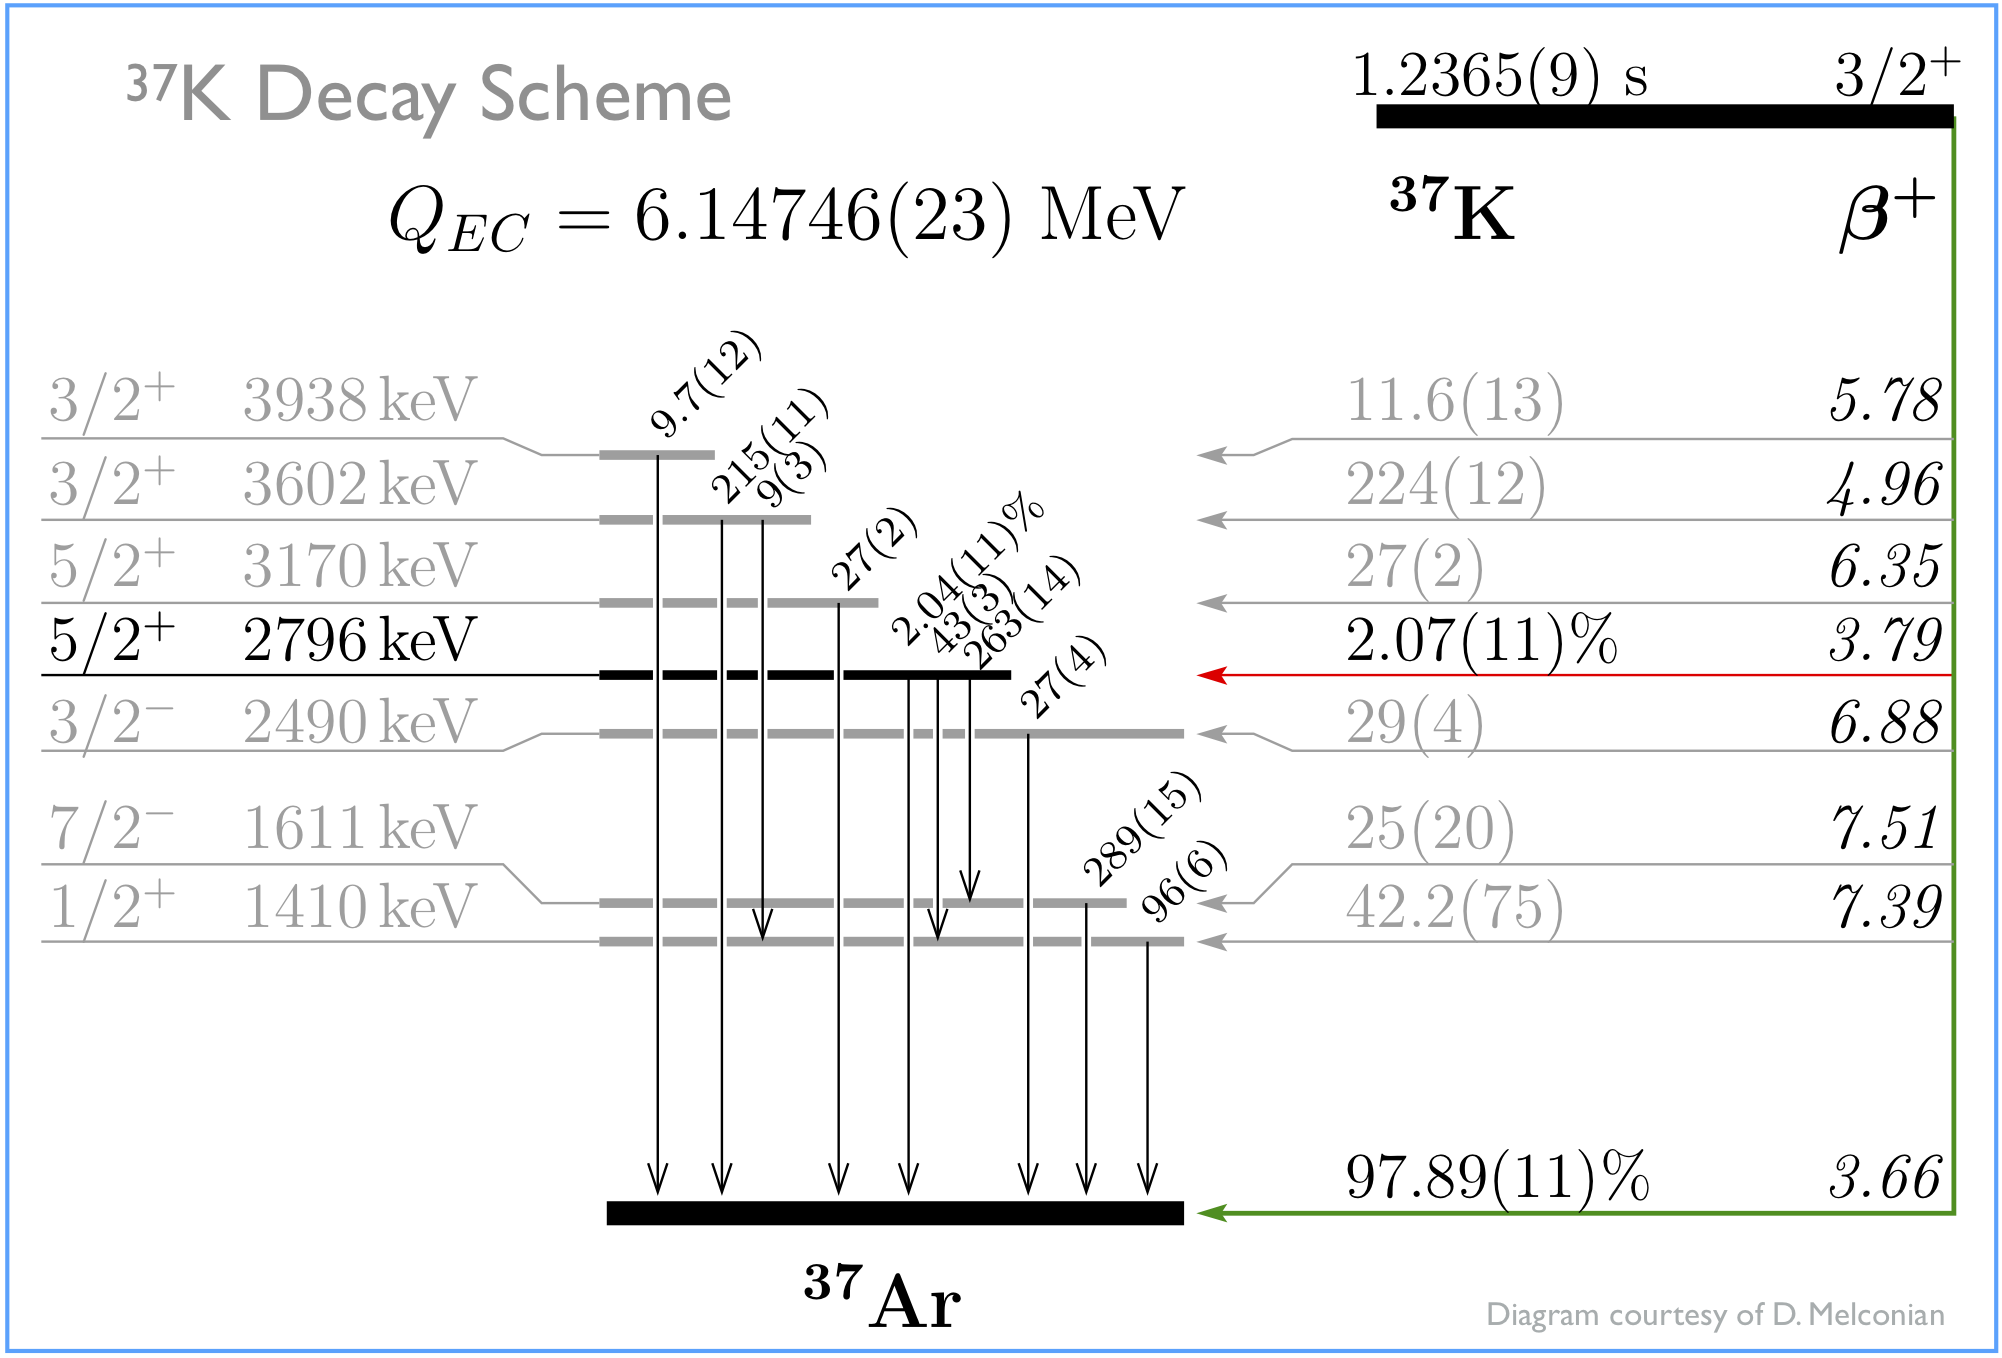
\includegraphics[width=.999\linewidth]
	{Figures/NuclearLevelDiagram.png}
	\note[jbn]{The caption should include that the right-hand column is log\_10(fT), a measure of the absolute decay rate (ref. Krane e.g.).
the left-hand column has $I^\pi$ where I is spin and $\pi$ is parity. This should not only include Dan's thesis for a reference, but the most recent paper with the branches-- it should work to reference P.D. Shidling
et al. Phys Rev C 98 015502 (2018) which re-did the half-life and summarized the fT value extraction. I see no publication of your branching ratio work, so I referenced Ozmetin's DNP talk in an earlier note.
}
	\caption{A level diagram for the decay of $\isotope[37]{K}$.}	
	\label{fig:nuclearleveldiagram}
\end{figure}


As in any decay, the angular correlations between the emerging daughter particles provide a rich source of information about the type of interaction that produced the decay.  
This particular decay involves a set of `mirror' nuclei, meaning that the nuclear wavefunctions of the parent and daughter are identical up to their isospin quantum number and corresponding electrical charge.~\aside[jbn]{no one will let you publish air quotes, ever. Have mercy on your committee, take them all out.  Use the opportunity to make sure you've defined them.
\\...\\
Here, just say isobaric mirror nuclei. You define it right there in text. It's fine to use textbook terms as long as you define them immediately.} \noindent
Because the two wavefunctions are so similar, effects to the decay from nuclear structure corrections can be kept to a minimum, and it is therefore possible to place especially strong constraints on the size of the theoretical uncertainties associated with the decay.  \aside[bluetodo]{Is it definitely true that the nuclear structure corrections are *smaller*?  Or is it just that they're better understood?}


%As a result, observations of this particular decay can be used to place especially strong constraints on 
%This property allows us to place strong constraints on the size of the theoretical uncertainties for this decay process within the Standard Model.  

%\note{ ``Of particular interest is the decay process: $^{37}\textrm{K} \rightarrow \,^{37}\textrm{\!Ar} + \beta^{+} + \nu_e$.  Among other useful properties, this is is a `mirror' decay, meaning that the nuclear wavefunctions of the parent and daughter are identical up to their isospin quantum number.  
%%the number of protons in the parent nucleus (19) is equal to the number of neutrons in the daughter, and the number of neutrons in the parent (18) is equal to the number of protons in the daughter.  
%This property allows us to place strong constraints on the size of the theoretical uncertainties for this decay process within the Standard Model.   %We further exploit this property by noting that both the $^{37}\textrm{K}$ parent and the $^{37}\textrm{\!Ar}$ daughter have nuclear spin $I=3/2$, a fact which is key to this experiment.
%''}


%\note{Talk about how great \isotope[37]{K} is for what we're doing with it.  Also, drop all the math-numbers to support those assertions.  Reference the level diagram within the text!}

\note{Also, 37K is a really nice isotope for this, because 
%98\% + 2\%, 
%also because it's a mirror decay, 
%also because it's an alkali.  Also-
%also, 
its big $\Abeta$ value means we have a big thing to multiply any $\bFierz$ value there might be when we construct the superratio asymmetry to eliminate systematics.}

%\missingfigure{This thing is going to need a nuclear level diagram for 37K.  Also, 37K is a really nice isotope for this, because 98\% + 2\%, also because it's a mirror decay, also because it's an alkali.  Also-also, its big $\Abeta$ value means we have a big thing to multiply any $\bFierz$ value there might be when we construct the superratio asymmetry to eliminate systematics.}


%\section{Exotic Couplings}
%%	In particular, we're interested in so-called scalar and tensor couplings within the nuclear weak force. Standard model beta decay involves only vector and axial-vector couplings, combined with a ``$(V-A)$'' handedness (left-handed).  



%%%% --- * --- %%%%	
\section{The Shake-off Electron Spectrum}
\label{section:soe_intro}
Although the beta decay process is primarily concerned with the emission of beta particles (electrons or positrons) from a Weak interaction that occurs within the nucleus, it is common for one or more \emph{orbital} electrons to also be lost in the process.  Although beta particles are emitted over a continuous energy spectrum, they commonly carry several MeV of kinetic energy.  By contrast, an atomic electron that becomes unbound in this process is likely to only carry a few eV of kinetic energy, and we say that they are `shaken' off.  
\note[jbn]{These are referred to as shakeoff electrons (SOEs), since they are in some sense shaken off.}

We will amend Eq.~\ref{eq:ourdecay} to reflect the presence of $N$ such `shake-off electrons' (SOEs) within each decay event, as
\bea
^{37}\textrm{K} &\rightarrow& \,^{37}\textrm{\!Ar}^{(N-1)+} + \beta^{+} + \nu_e + N \, e_{\textrm{SO}}, 
\label{eq:ourdecay_withsoe}
\eea
%\aside{Do I want to re-assign N somehow so the notation works better?}
where it is clear that, since the parent $^{37}\textrm{K}$ atom was electrically neutral before its decay by $\beta^+$ emission, the daughter $^{37}\textrm{\!Ar}$ will initially have an `extra'~\aside[jbn]{'extra' -> extra. You're not breaking charge conservation here, you don't need to define the word.} orbital electron (and therefore a negative net charge) if no electrons are shaken off.  We also note that it is common for multiple SOEs to be created in a given decay event.  

A further consideration is that the outer electron in an $^{37}\textrm{\!Ar}^{-}$ ion is \emph{not bound},~\aside{cite someone!!  I don't know who.} and in an electric field such as is present within our experimental chamber, this outer electron is removed immediately to be accelerated through the field, leaving behind a neutral $^{37}\textrm{\!Ar}$ atom.  Although this is in principle a different physical loss mechanism, we will refer to unbound electrons resulting from either process as SOEs.  

It is useful to consider the energy spectrum of these shake-off electrons.  The most straightforward component of the SOE energy spectrum arises from the electrons that are lost immediately following decay, and we take these to initially have 0eV in kinetic energy.  

For the shake-off electrons arising from the Weak process itself, the initial energy spectra for SOEs originating in a particular orbital shell can be estimated according to the procedure outlined by Levinger~\cite{Levinger}.
~\note[jbn]{$\rightarrow$``by Levinger, who credits Feynman for the suggestion~\cite{Levinger}.''
\\...\\
(Since this is a true story that is not embellished by Feynman in someone else's joke book, but is in a footnote in the Physical Review,  I like to mention it.)
}  \noindent
The strategy is to assume that the sudden approximation holds, and simply calculate the overlap in electron wavefunctions between the initial and final states, where the final state may be either an outgoing electron or one bound within the atom.  Analytic expressions can be obtained if the atom is treated as being hydrogenic -- an excellent approximation here, as $^{37}\textrm{K}$ is an alkali.  

Unfortunately, this treatment cannot determine the fractional contribution of each orbital to the total, nor can it determine the \emph{number} of electrons likely to be removed in a single decay event.  The implications of the SOE energy spectrum to the present experiment are discussed further in Section~\ref{sec:tof_bg}.

\note[bluetodo]{In the end, we used $(0.09)*(\textrm{0eV}) + (0.91)*(0.85*(\textrm{4S}) + 0.15*(\textrm{3P}))$.  But I say that in the other section.  Also, John used Eq.20 for the 4S, and Eq.24 for the 3P.}
\note{Comment on how well this matches our data?  Somehow?}

%\note{Should I talk about the distribution of how many SOEs come off in a decay?  I have measurements of the recoil charge distribution, which is related but not really the same thing.  From a theoretical POV, I don't know how many get shaken off.  Thankfully, it doesn't matter very much in the end.}

%%%%%\begin{figure}[h!!t]
%%%%%	\centering
%%%%%	\includegraphics[width=.999\linewidth]
%%%%%	{Figures/Levinger_SOETOF_prelim.pdf}
%%%%%	\note[clean]{Clean up SOE TOF pic in intro.  It doesn't show what I need!}
\note{A picture of the SOE spectrum for the intro was here.  It's gone now, but it's important that we remember!}
%%%%%	\note{Maybe just kill this picture?  At least reference it in the text somewhere.}
%%%%%	\caption[Levinger TOF]{Shake-off electron TOF (w.r.t. beta TOA) spectrum, showing how the spectrum is different if one includes different sets of initial electrons to be shaken off.  I forget why some of them have 0 eV.  Maybe those are the ones from the $\isotope[37]{Ar}^+$. ... Levinger TOF spectra for some different sets of SOE initial orbitals before shake-off.  (At least that's what it's supposed to be, after I fix the picture).  It's reconstructed event-by-event with beta times-of-flight that would pass some basic `good event' cuts.  Anyway, it turns out, it doesn't much matter what orbitals you lose SOEs from.  That's nice.  In the end, I used 85+15.  \comment{(Need to re-plot this.)} }	
%%%%%	\label{fig:levinger_TOF}
%%%%%\end{figure}


%%%% --- * --- %%%%
\FloatBarrier  % This will have to go away later.
\section{Fierz Interference -- The Physical Signature}
\label{signature_chapter}
The physical effects resulting from the presence of scalar or tensor couplings include a small perturbation to the energy spectrum of betas produced by radioactive decay, labeled $\bFierz$ in Eq.~\ref{equation:integrated_jtw}.  Within the Standard Model, the parameter $\bFierz$ is identically zero, and a departure from that would be indicative of (BSM) scalar or tensor couplings.  

The measured value of $\bFierz$ can be evaluated by using a simple beta energy spectrum, as in the top plot of Fig.~\ref{fig:FierzSignature}, but by~\aside[jbn]{$\rightarrow$ not only by.... but also by...} constructing a so-called ``superratio asymmetry'' instead (bottom plot in Fig.~\ref{fig:FierzSignature}), these small changes to the overall spectrum are amplified, and many systematic effects cancel out entirely.  This result comes at the cost of an increased statistical uncertainty.
\note[jbn]{By normalizing Eq.~\ref{equation:integrated_jtw_INTRODUCTION} to have a conventional angular distribution 1 + (term)*$\Abeta$, we can write 
$W(\theta) = 1 + \Abeta/(1+\bFierz \E/\me) cos(\theta) 
\approx 
1 + \Abeta cos(\theta) - \bFierz \E/\me \Abeta cos(\theta) $
for small $\bFierz$.
Our  superratio observable measures directly the coefficient of the $cos(\theta)$ term., and its distortion with energy is multiplied by $\bFierz \Abeta$.
\\...\\
The 37K $\Abeta$ is much larger than the neutron's $\Abeta$, so we gain in sensitivity compared to the neutron.
}
\begin{figure}[h!!t]
	\centering
	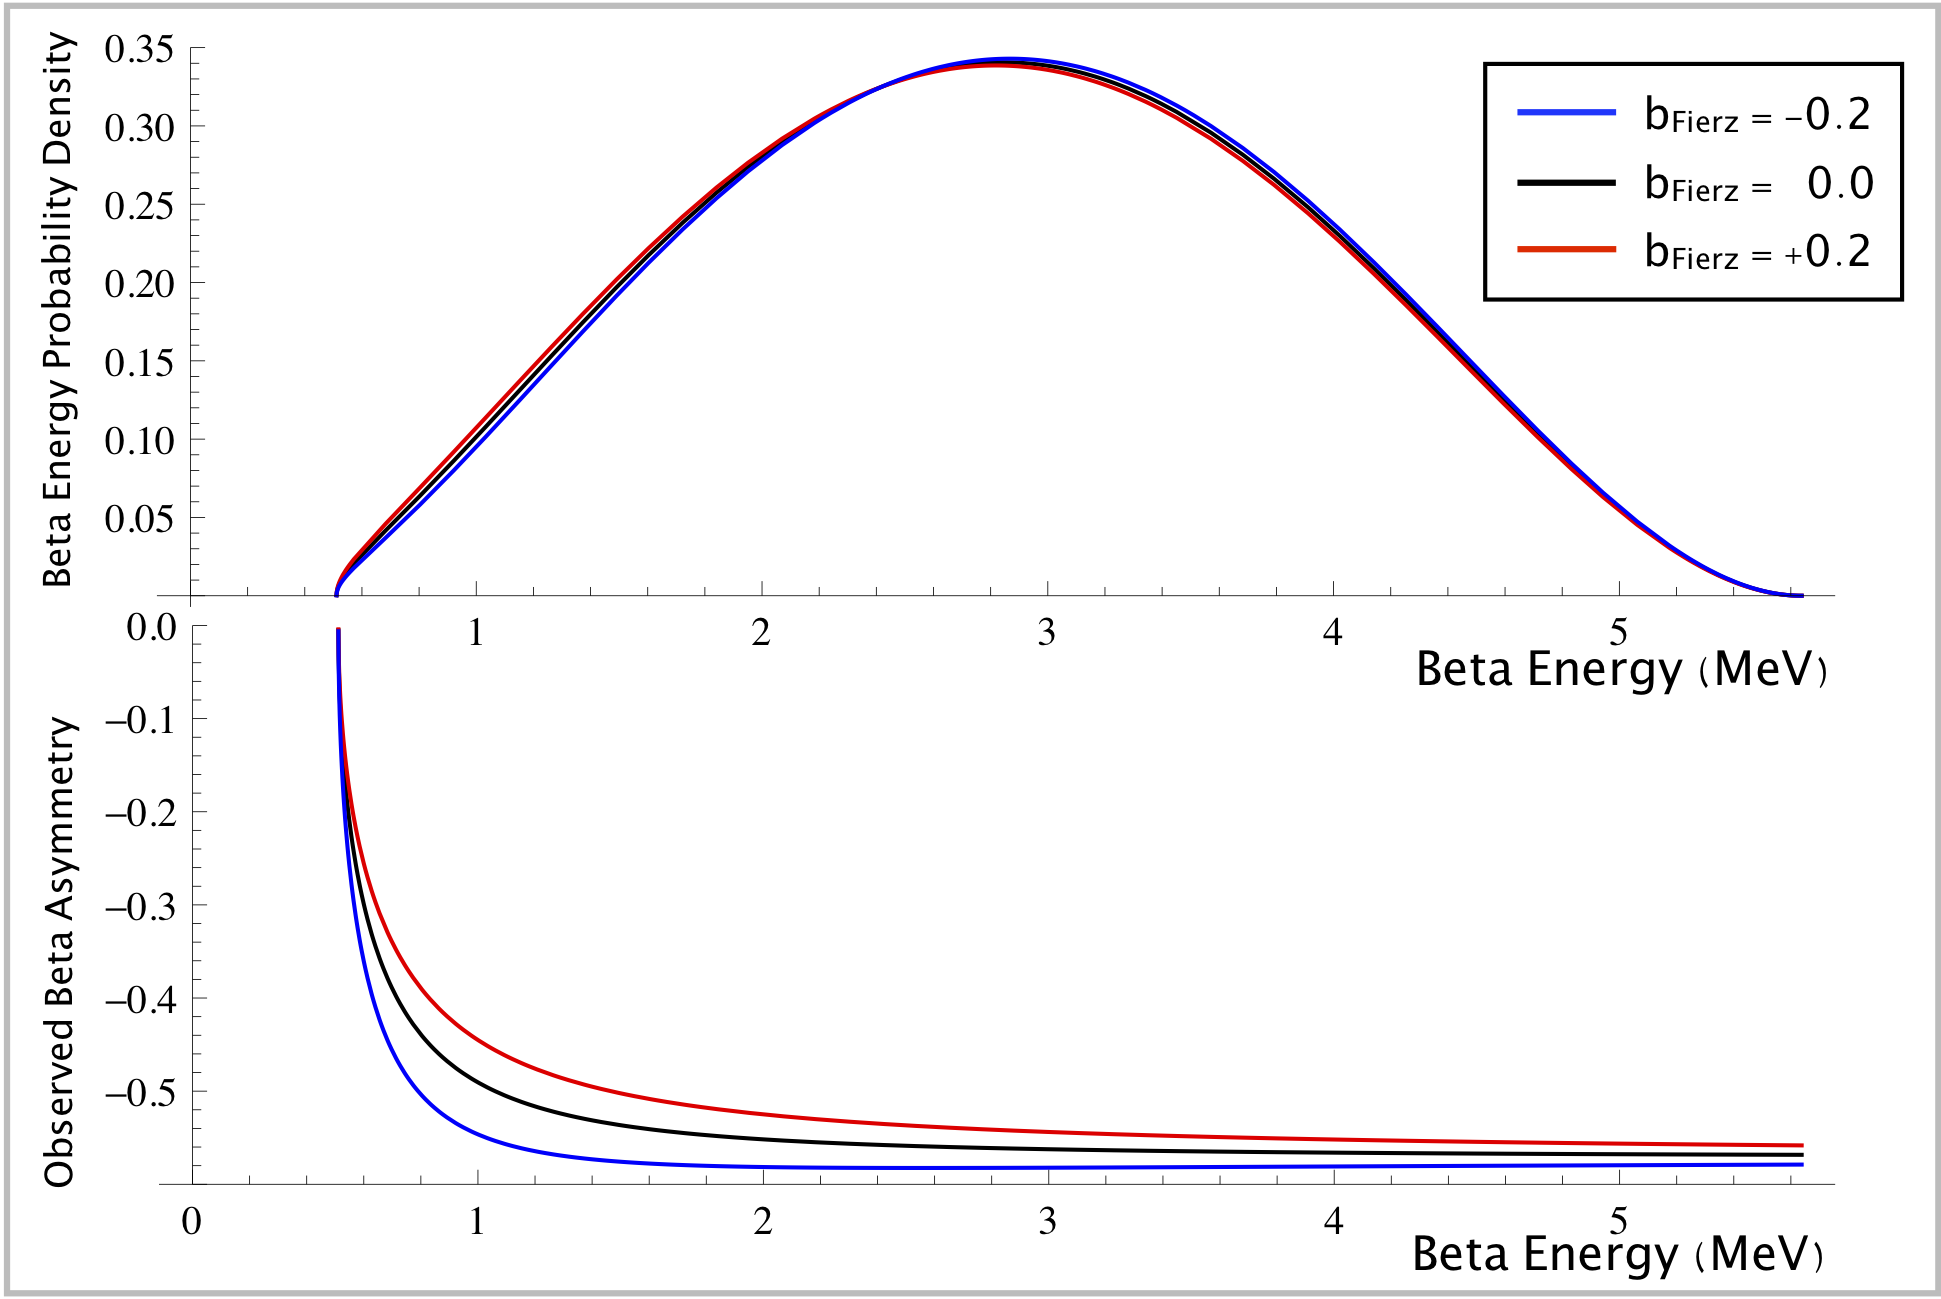
\includegraphics[width=.999\linewidth]
	{Figures/Fierz_Signature.png}
	\caption[Naive Beta Energy Spectrum and Superratio Asymmetry to Measure $\bFierz$]{A naive beta energy spectrum (top) and superratio asymmetry (bottom) are constructed to measure $\bFierz$.}	
	\label{fig:FierzSignature}
\end{figure}

The superratio and superratio asymmetry are discussed in detail in Appendix~\ref{appendix:superratio}.  The discussion includes details on which sort of systematic errors will cancel out entirely, or to leading order, with this treatment -- however it must be noted that for this project, higher-order corrections are included in all simulations, and the effects are propagated through to the end of the analysis.  Therefore, measured values of $\Abeta$ (and $\bFierz$, though that is trivial) may be directly compared to theoretical predictions.  

%%%, and the sort of systematic errors that cancel out under this treatment are discussed in detail in Appendix~\ref{appendix:superratio}.


\note{the "Physical Signature" section probably needs more work, but it's not getting it tonight.}
\note[jb1]{JB on simple things still missing:
\\
Intro or theory section:
\\...\\
P(cos(theta)) = 1 + bm/E + P  Abeta v/c cos(theta)
\\
where theta is the angle between beta and polarization direction
\\...\\
Higher-order corrections to this equation (citing your appendices and/or
chapters) are included in the simulation,
so you are extracting b and Abeta in this
equation to be compared with theory
\\...\\
\{This is a simple but vital statement-- some people actually extract Abeta(Ebeta$=$0) without recoil-order corrections, which is not the same parameter.\}
\\...\\
The theory prediction for Abeta (citing Fenker PRL) is X.
\\
The theory prediction for bFierz is 0 (maybe you have that already).
}

%\note[jb1]{JB:  ``I doubt I will have further useful comments on the Ch. (((this chapter))) as they are now.'' }

%\missingfigure{I need that simulated picture of the different beta energy spectra, with different values of $\bFierz$.}
\note[jb1]{JB on that missing figure that I've now put in:    ``A dependence of Abeta on beta energy is also introduced.
\\
UCNA fits energy spectrum and Abeta[Ebeta] simultaneously now."
}

%\section{Present Limits}
%	A bit about other people's physics.

\note{The point is, the presence of either scalar or tensor interactions will produce a $\bFierz$ term in the decay PDF.  It has other effects on the PDF, but those come in at higher-order in the tiny scalar and tensor couplings.  So, the Fierz term would be by far the biggest thing that changes in the PDF.  The PDF describes the energy and momentum of the outgoing beta w.r.t. a variety of other things.  Notably, we can write an elegant-ish description of beta momentum w.r.t. nuclear polarization direction, and ignore the neutrino completely after integrating over it.  We have a PDF in beta \emph{direction} (w.r.t. polarization), and beta \emph{energy}.  To lowest order (and lowest order is best order) the distribution w.r.t. polarization direction doesn't change, but the distribution w.r.t. energy does change.  Or ... something?  The point is, it makes a change in the beta energy spectrum.  This change is most pronounced at low energies, because the Fierz term is scaled by $(1/\Ebeta)$.  However, the asymmetry is also a function of $\Ebeta$.  A different function of $\Ebeta$.  In fact, it is scaled by $(\pbeta/\Ebeta)$ within the PDF, which is distinctly different than $\bFierz$.  So, one might ask what effect a $\bFierz$ term would produce on a constructed asymmetry spectrum.  ....This explanation has gone way off track.}

\note{Here's a reference to the picture that shows the result of a non-zero $\bFierz$ term.  It's Fig.~\ref{fig:FierzSignature}.}



\note{Kludge-deleted section:  ``On the Superratio, the Supersum, and the Constructed Asymmetry''}
%\section{On the Superratio, the Supersum, and the Constructed Asymmetry}
\note{Clean Superratio,Supersum,Super-Asymmetry section.  Prolly merge w/ bFierz section.}
\note[jb1]{JB:  You need to at some point say that the supersum is the beta energy spectrum.  There are experiments trying to do this method better, but they are very difficult.  UCNA published a combined energy spectrum and Abeta[Ebeta] analysis on the neutron in March 2020~\cite{NeutronbFierz_March2020}.
\\...\\
MJA:  I can't help but also notice the follow-up article from September 2020~\cite{Saul2020}.  Ugh. 
}

%\\*
The data can be combined into a superratio asymmetry.  This has the benefit of causing many systematics to cancel themselves out at leading order.  It also will increase the fractional size of the effects we're looking for.  This can be shown by using math.~\aside[jbn]{``This is shown in full detail in Appendix~\ref{appendix:superratio}.''}

%\\*
Not all systematics effects are eliminated.  We'll want to be careful to propagate through any effects that are relevant.  Using the superratio asymmetry as our physical observable makes this process a bit messier for the things that don't cancel out, but it's all just math.
~\aside[jbn]{You really need a literature reference to the superratio method here. I know you have one. Danny gave us one a long time ago.
}
Some other groups have performed similar measurements using the supersum as the physical observable.  There are pros and cons to both methods.  I can show, using a back-of-the-envelope calculation, that for this particular dataset, the superratio asymmetry method produces a better result.  
\note[jbn]{If you're not going to do this back-of-envelope calculation here, you need to just reference Appendix D and likely eliminate this paragraph?}

